\documentclass[a4paper,12pt]{ETHexercise}
\usepackage{bbm}

\input{preamble}

\usepackage{multirow}
\title{NLP Assignment}
\begin{document}
\setserie{1}


\newcommand{\pair}[2]{{\langle #1 , #2 \rangle}}
\newcommand{\score}[2]{\text{score}(#1, #2, \mathbf{w})}

\lectureheader{Prof. Ryan Cotterell}
{}
{\Large Natural Language Processing}{Fall 2022}
\begin{center}
  {\Huge Simon Wachter: Assignment 2}\\
  \quad\newline
  siwachte@ethz.ch, 19-920-198\\
  \quad\newline
  \timestamp
\end{center}

\begin{question}\\
  \begin{subquestion}
    Prove that the expectation semiring satisfies the semiring axioms:\\
    \begin{itemize}
      \item  $(\R \times \R, \oplus, \mathbf{0})$ must be a commutative monoid with identity element $\mathbf{0}$:
            \begin{align}
              \left(\pair{x}{y} \oplus \pair{x'}{y'}\right) \oplus \pair{x''}{y''} & =       \pair{x + x'}{y + y'}      \oplus \pair{x''}{y''}              \\
                                                                                   & = \pair{x + x' + x''}{y + y' + y''}                                    \\
                                                                                   & = \pair{x}{y} \oplus \pair{x' + x''}{y' + y''}                         \\
                                                                                   & = \pair{x}{y} \oplus \left(\pair{x'}{y'} \oplus \pair{x''}{y''}\right)
            \end{align}
            \begin{align}
              \mathbf{0} + \pair{x}{y} & = \pair{0}{0} \oplus \pair{x}{y} \\
                                       & = \pair{0 + x}{0 + y}            \\
                                       & = \pair{x}{y}                    \\
                                       & = \pair{x + 0}{y + 0}            \\
                                       & = \pair{x}{y} + \mathbf{0}
            \end{align}
            \begin{align}
              \pair{x}{y} + \pair{x'}{y'} & = \pair{x + x'}{y + y'}       \\
                                          & = \pair{x' + x}{y' + y}       \\
                                          & = \pair{x'}{y'} + \pair{x}{y}
            \end{align}
      \item $(\R \times \R, \otimes, \mathbf{1})$ must be a monoid with identity element $\mathbf{1}$:
            \begin{align}
              \left(\pair{x}{y} \otimes \pair{x'}{y'} \right) \otimes \pair{x''}{y''} & = \pair{x \cdot x'}{x \cdot y' + y \cdot x'} \otimes \pair{x''}{y''}                              \\
                                                                                      & = \pair{x \cdot x' \cdot x''}{x \cdot x' \cdot y'' + (x \cdot y' + y \cdot x') \cdot x''}         \\
                                                                                      & = \pair{x \cdot x' \cdot x''}{x \cdot x' \cdot y'' + x \cdot y' \cdot x'' + y \cdot x' \cdot x''} \\
                                                                                      & = \pair{x}{y} \otimes \pair{x' \cdot x''}{x' \cdot y'' + y' \cdot x''}                            \\
                                                                                      & = \pair{x}{y} \otimes \left(\pair{x'}{y'} \otimes \pair{x''}{y''}\right)
            \end{align}
            \begin{align}
              \mathbf{1} \otimes \pair{x}{y} & = \pair{1}{0} \otimes \pair{x}{y} \\
                                             & = \pair{1 \cdot x}{1 \cdot y}     \\
                                             & = \pair{x}{y}                     \\
                                             & = \pair{x \cdot 1}{y \cdot 1}     \\
                                             & = \pair{x}{y} \otimes \mathbf{1}
            \end{align}
      \item Multiplication left and right distributes over addition:
            \begin{align}
              \pair{x}{y} \otimes \left(\pair{x'}{y'} \oplus \pair{x''}{y''}\right) & = \pair{x}{y} \otimes \pair{x' + x''}{y' + y''}                                                          \\
                                                                                    & = \pair{x \cdot x' + x \cdot x''}{x \cdot y' + x \cdot y'' + y \cdot x' + y \cdot x''}                   \\
                                                                                    & = \pair{x \cdot x'}{x \cdot y' + y \cdot x'} \oplus \pair{x \cdot x''}{x \cdot y'' + y \cdot x''}        \\
                                                                                    & = \left(\pair{x}{y} \otimes \pair{x'}{y'}\right) \oplus \left(\pair{x}{y} \otimes \pair{x''}{y''}\right)
            \end{align}
            \begin{align}
              \left(\pair{x}{y} \oplus \pair{x'}{y'}\right) \otimes \pair{x''}{y''} & = \pair{x + x'}{y + y'} \otimes \pair{x''}{y''}                                                              \\
                                                                                    & = \pair{x \cdot x'' + x' \cdot x''}{x \cdot y'' + x' \cdot y'' + y \cdot x'' + y' \cdot x''}                 \\
                                                                                    & = \pair{x \cdot x''}{x \cdot y'' + y \cdot x''} \oplus \pair{x' \cdot x''}{x' \cdot y'' + y' \cdot x''}      \\
                                                                                    & = \left(\pair{x}{y} \otimes \pair{x''}{y''}\right) \oplus \left(\pair{x'}{y'} \otimes \pair{x''}{y''}\right)
            \end{align}
      \item Multiplication by $\mathbf{0}$ annihilates $\R \times \R$:
            \begin{align}
              \mathbf{0} \otimes \pair{x}{y} & = \pair{0}{0} \otimes \pair{x}{y}       \\
                                             & = \pair{0 \cdot x}{0 \cdot y}           \\
                                             & = \pair{0}{0}                           \\    &= \mathbf{0}         \\
                                             & = \pair{0}{0}                           \\
                                             & = \pair{x \cdot 0}{y \cdot 0}           \\
                                             & =       \pair{x}{y} \otimes \pair{0}{0} \\
                                             & = \pair{x}{y} \otimes \mathbf{0}
            \end{align}
    \end{itemize}
  \end{subquestion}
  \begin{subquestion}
    Our initial graph looks like \cref{figure:graph}.
    \begin{figure}[H]
      \centering
      \label{figure:graph}
      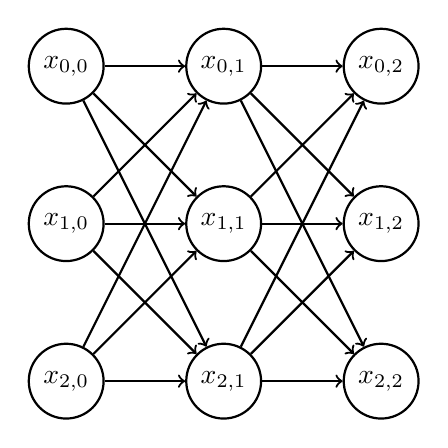
\begin{tikzpicture}[node distance={20mm}, thick, main/.style = {draw, circle}]
        \node[main] (0) {$x_{0,0}$};
        \node[main] (1) [below of=0]{$x_{1,0}$};
        \node[main] (2) [below of=1]{$x_{2,0}$};

        \node[main] (3) [right of=0]{$x_{0,1}$};
        \node[main] (4) [below of=3]{$x_{1,1}$};
        \node[main] (5) [below of=4]{$x_{2,1}$};

        \node[main] (6) [right of=3]{$x_{0,2}$};
        \node[main] (7) [below of=6]{$x_{1,2}$};
        \node[main] (8) [below of=7]{$x_{2,2}$};

        \draw[->] (0) -- (3);
        \draw[->] (0) -- (4);
        \draw[->] (0) -- (5);

        \draw[->] (1) -- (3);
        \draw[->] (1) -- (4);
        \draw[->] (1) -- (5);

        \draw[->] (2) -- (3);
        \draw[->] (2) -- (4);
        \draw[->] (2) -- (5);

        \draw[->] (3) -- (6);
        \draw[->] (3) -- (7);
        \draw[->] (3) -- (8);

        \draw[->] (4) -- (6);
        \draw[->] (4) -- (7);
        \draw[->] (4) -- (8);

        \draw[->] (5) -- (6);
        \draw[->] (5) -- (7);
        \draw[->] (5) -- (8);

      \end{tikzpicture}
      \caption[]{The initial graph}
    \end{figure}
    Where the columns represent the words in $\mathbf{w}$ and the rows represent different tags.
    In this non lifted graph, our forward propagation will yield the following values, when using the score functions as edge weights in the graph:
    \begin{align}
      z_{i,j} & = \sum_{k=0}^{T} (z_{k,j-1} \cdot \score{x_{k, j-1}}{x_{i,j}})
    \end{align}
    Where we used the algorithm from the script:
    \begin{algorithm}
      \SetAlgoLined
      \caption{Forward pass}
      \label{algo:forward}
      $\beta(\mathbf{w}, t_0) = 1$\\
      \For{$n = 1 \to N$}{
        $\beta(\mathbf{w}, t_n) = \sum_{t_{n-1} \in \mathcal{T}} \exp(\score{\langle t_n}{t_{n-1}\rangle}) \otimes \beta(\mathbf{w}, t_{n-1})$
      }
    \end{algorithm}
    When we now lift the CRF into the expectation semiring, the forward propagation algorithm changes to:\\
    \begin{algorithm}[H]
      \SetAlgoLined
      \caption{Forward pass}
      \label{algo:forward_semi}
      $\beta(\mathbf{w}, t_0) = \langle 1, 0 \rangle$\\
      \For{$n = 1 \to N$}{
        $\beta(\mathbf{w}, t_n) = \oplus_{t_{n-1} \in \mathcal{T}} \langle w, -w \log w \rangle \otimes \beta(\mathbf{w}, t_{n-1})$
      }
    \end{algorithm}
    Where $w = \exp(\score{\langle t_n}{t_{n+1}\rangle})$.\\
    We want to show that the result of the forward propagation lifted in the semiring is the same as the unnormalized Entropy:
    \begin{align}
      H_u(T_{w}) & = -\sum_{\mathbf{t} \in \mathcal{T}^N} \exp(score_{\boldsymbol{\theta}} (\mathbf{t},\boldsymbol{w})) score_{\boldsymbol{\theta}} (\mathbf{t},\boldsymbol{w}) \\
    \end{align}

    We show this by induction
  \end{subquestion}
\end{question}
\end{document}

%%% Local Variables:
%%% mode: latex
%%% TeX-master: t
%%% End: